\section{Analysis strategy}
\label{sec:Durchführung}
This analysis is done with three data samples of which the invariant mass distributions are shown in \autoref{fig:dists}. Two of those contain Monte Carlo (MC) simulation of the $B^0_s \to \psi(2S)K^0_\mathrm{S}$ and the kinematically similar $B^0_d \to \psi(2S)K^0_\mathrm{S}$ decay, respectively. The third data sample contains data recorded by the LHCb experiment.
The simulation of the $B^0_d$ decay will be used as a control channel.
Since the $B^0_d$ signal can be extracted from the data it can be compared to its MC simulation allowing to select features that are well described in the simulation. Because the $B^0_d$ and the $B^0_s$ decay are so similar kinematically one can assume that these features are also described well in the $B^0_s$ MC simulation.
To select a small number of features with a high seperation power between signal and background the data is compared to the $B^0_s$ simulation afterwards.
The remaining features are used to implement a BDT that serves as a multivariate classifier to reject as much combinatorial background as possible. For trianing it is provided the $B^0_s$ simulation a signal and a part of the data as background samples.
A fit model is applied to the selected data. The parameters describing the two peaks are obtained from fits to the simulations beforehand.
From the fit model the signal yield can be determined and the statistical significance can be estimated.

\begin{figure}[tb]
  \centering
  \begin{subfigure}{.32\textwidth}
    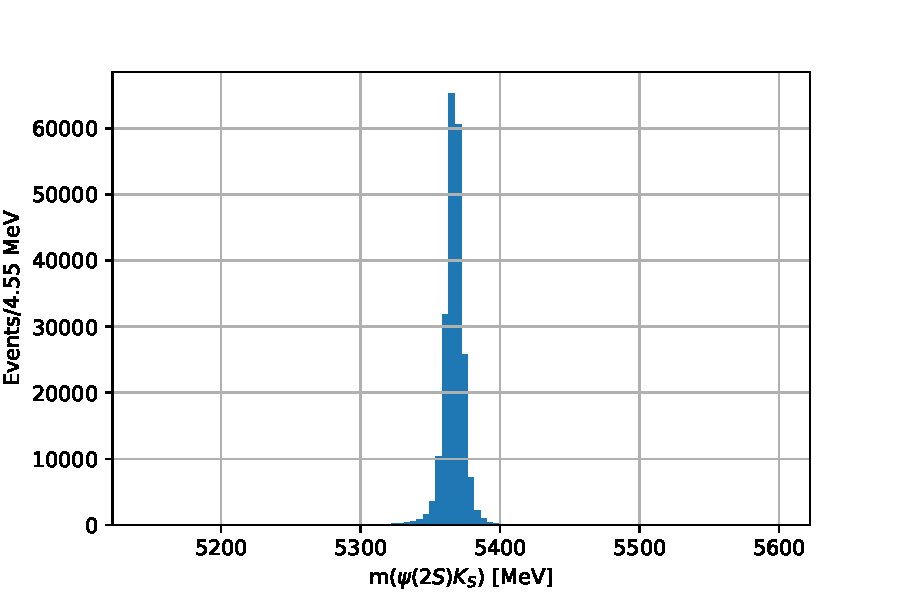
\includegraphics[width=\linewidth]{plots/sim_hist.pdf}
  \end{subfigure}
  \begin{subfigure}{.32\textwidth}
    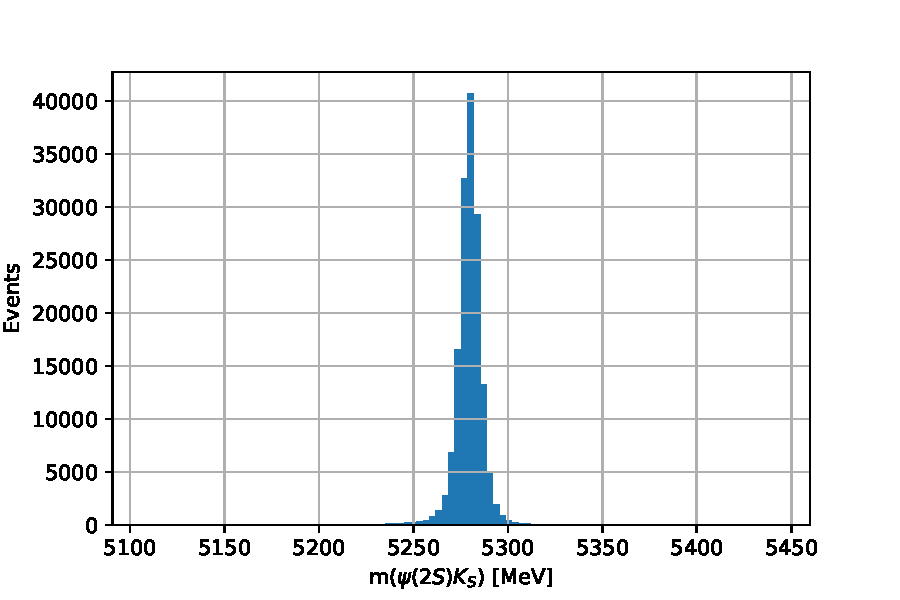
\includegraphics[width=\linewidth]{plots/control_sim_hist.pdf}
  \end{subfigure}
  \begin{subfigure}{.32\textwidth}
    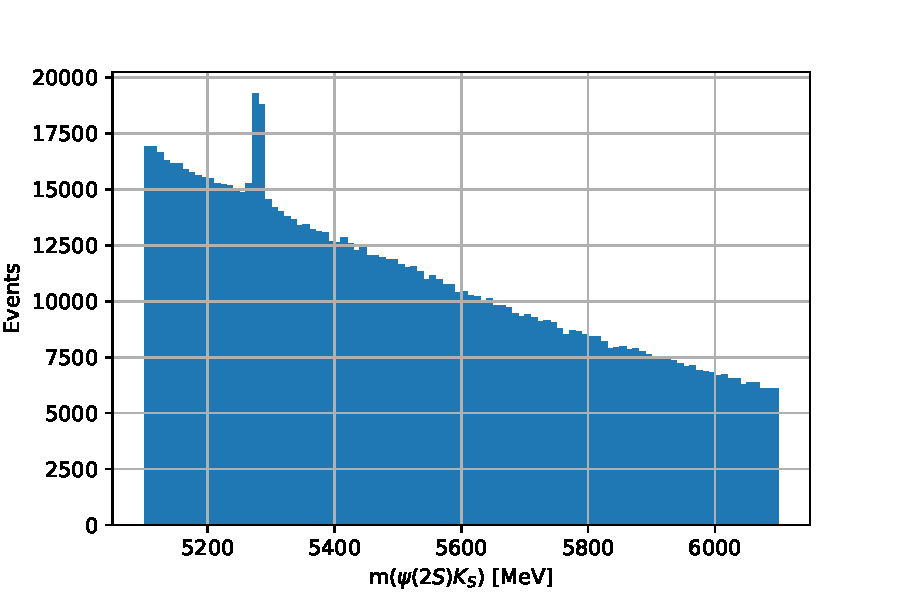
\includegraphics[width=\linewidth]{plots/data_hist.pdf}
  \end{subfigure}
  \caption{Invariant mass distributions of the MC simulated decays $B^0_s$ (left) and $B^0_d \to \psi(2S) K^0_\mathrm{S}$ (middle), as well as recorded data from the LHCb experiment (right).}
  \label{fig:dists}
\end{figure}
